\section{深度神经网络}
深度神经网络包括卷积神经网络和循环神经网络。卷积神经网络一般应用于计算机视觉,循环神经网络一般应用于自然语言处理。近年来,两者发展都很快,并且相互借鉴。
\subsection{卷积神经网络}
\paragraph{LeNet}\cite{lecun1998gradient}由Yann LeCun于1998年提出,是第一种实用的卷积神经网络,广泛用于手写字符识别。如图\ref{fig:lenet},LeNet网络结构简单,仅包括7层,但是包含了深度学习的基本模块:卷积层、池化层、全连接层,是所有卷积神经网络的基础。LeNet在minst数据集上取得了较好的结果,但是限于硬件算力与软件算法限制,没有应用于更加复杂的计算机视觉问题。
\begin{itemize}
\item 输入层的大小为32*32*3(三通道)
\item C1是卷积层,使用6个大小为5*5的卷积核,得到28*28*6的特征图
\item S2是池化层,步长为2,得到14*14*6的特征图
\item C3层是卷积层,通过对S2的输出特殊组合,得到10*10*16的特征图
\item S4是池化层,得到5*5*16的特征图
\item C5是卷积层,使用120个5*5的卷积,得到1*1*120的特征图
\item F6是全连接层,有84个节点
\item 输出层是全连接层,有10个节点(代表数字0-9)
\end{itemize}
\begin{figure}
    \centering
    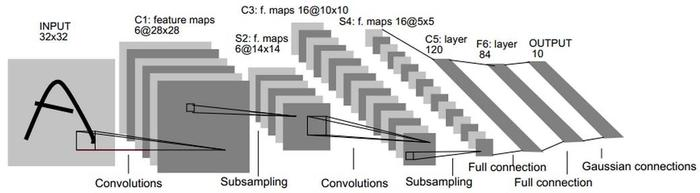
\includegraphics[width=0.7\linewidth]{AI/figures/LeNet.jpg}
    \caption{LeNet}
    \label{fig:lenet}
\end{figure}

\paragraph{AlexNet}\cite{krizhevsky2012imagenet}由Hinton及其学生于2012年提出,夺得当年ILSVRC比赛冠军,其错误率远低于已有算法。如图\ref{fig:alexnet},AlexNet在现有深度神经网络上做了大量改进,包括:使用ReLU\cite{glorot2011deep}代替Sigmoid作为激活函数,解决了神经网路深层梯度消失问题;使用Dropout\cite{srivastava2014dropout,tinto1975dropout}避免过拟合;用最大池化\cite{nagi2011max}取代平均池化,提高特征丰富性;提出局部响应归一化(Local Respone Normalization,LRN)层,增强模型泛化能力;使用CUDA和双路并行网络设计,显著加速训练;采用数据增强,减小过拟合、提高泛化能力。
\begin{figure}
    \centering
    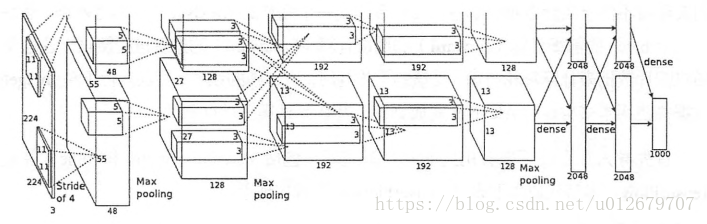
\includegraphics[width=0.7\linewidth]{AI/figures/AlexNet.png}
    \caption{AlexNet}
    \label{fig:alexnet}
\end{figure}

\paragraph{GoogLeNet}\cite{szegedy2015going}由Google公司于2014年首次提出,有多个升级版本。为有效增加模型深度(网络层数)和宽度(神经元数量),GoogLeNet提出多点创新:用多个1*1、3*3、5*5的小卷积核替代7*7的大卷积核;取消全连接层;在网络中大量使用Inception架构;增加辅助分类器。与AlexNet相比,GoogLeNet大幅增加了网络深度,同时减少了计算量和参数。

\paragraph{VGG}\cite{simonyan2014very}由Oxford Visual Geometry Group于2014年提出,和GoogLeNet一起在当年ILSVRC竞赛大放异彩。VGG比GoogLeNet参数多,但是在迁移到其它领域表现较优,常被其他领域用作基础网络。VGG结构简洁,卷积层均采用3*3的卷积核,池化层均采用2*2最大池化。

\paragraph{ResNet}\cite{he2016deep}即残差网络,由何凯明等人与2015年提出,获得当年ILSVRC多个视觉任务冠军,随即得到工业界和学术界的认可。在残差网络之前,深度神经网路一般不超过20层,更深的网络无法避免梯度消失等问题,难以训练。何凯明等人创造性的提出残差结构,打破顺序连接的惯例,将浅层输出跳跃式的输入深层,同时采用批标准化(Batch Normalization)\cite{ioffe2015batch}防止过拟合。通过这些改进,ResNet可以轻易超过上百层并且可以有效训练。残差网络的设计思路还被广泛应用于其他深度学习领域,均取得了较好的效果。

\subsection{循环神经网络}
循环神经网络(Recurrent Neural Network, RNN)主要用于处理上下文相关的问题,如自然语言处理。存在一类问题,其输入数据是一个序列,具有上下文依赖性。由于卷积神经网络前一个输入和下一个输入没有关联,处理此类问题效果不佳。而循环神经网络正是为了处理这类问题设计的,具有重复的结构。